% Uncomment this to make slides with overlays:
%\documentclass[slides]{beamer}

% Uncomment these (but comment the above \documentclass line) to make handouts:
\documentclass[handout]{beamer}

% Uncomment these to have more than one slide per page
\usepackage{pgfpages}
\pgfpagesuselayout{2 on 1}[border shrink=5mm]
\pgfpageslogicalpageoptions{1}{border code=\pgfusepath{stroke}}
\pgfpageslogicalpageoptions{2}{border code=\pgfusepath{stroke}}

\usepackage[]{graphicx, color, hyperref}

\mode<presentation>
{
	%\usetheme[secheader]{Boadilla}
	%\usecolortheme[rgb={.835, .102,.169}]{structure}  
	\usetheme[width= 0cm]{Goettingen}
	%\setbeamercovered{transparent}
}
\setbeamertemplate{navigation symbols}{}
\setbeamertemplate{footline}[frame number]

\definecolor{blue2}{rgb}{0.278,0.278,0.729} 
\newcommand{\blue}[1]{\textcolor{blue2}{#1}}
\newcommand{\white}[1]{\textcolor{white}{#1}}
\newcommand{\red}[1]{\textcolor{red}{#1}}
\newcommand{\xbar}{\overline{x}}
\newcommand{\ybar}{\overline{y}}
\newcommand{\phat}{\widehat{p}}
\newcommand{\prob}{\mbox{Pr}}
\newcommand{\E}{\mathbb{E}}
\newcommand{\Var}{\mbox{Var}}
\newcommand{\cp}{\oplus}
\newcommand{\cm}{\circleddash}


\title{Lecture 21: Difference of two proportions}
\author{Chapter 6.2}
\date{}


\begin{document}
%------------------------------------------------------------------------------
\begin{frame}
\titlepage
\end{frame}
%------------------------------------------------------------------------------


%------------------------------------------------------------------------------
\begin{frame}[fragile]
\frametitle{Question for today}

How do we infer about a difference in proportions $p_1-p_2$?

\end{frame}
%------------------------------------------------------------------------------


%------------------------------------------------------------------------------
\begin{frame}[fragile]
\frametitle{Surveys}

The way a question is phrased in survey can influence a person's response.  Ex on p.281: the Pew Research Center conducted a survey with the following question:

\pause\vspace{0.5cm}

\textit{By 2014 all Americans will be required to have health insurance.  \blue{X while Y}.  Do you approve of disapprove of this policy?}

\pause\vspace{0.5cm}

where $X$ and $Y$ were randomly ordered between
\begin{itemize}
\item People who do not buy insurance will pay a penalty
\item People who cannot afford it will receive financial help from the government
\end{itemize}

\vspace{0.5cm}

\pause Let's infer about the difference in proportion of people who \blue{approve}.

\end{frame}
%------------------------------------------------------------------------------


%------------------------------------------------------------------------------
\begin{frame}[fragile]
\frametitle{Example from Text}

\begin{small}
\begin{center}
  \begin{tabular}{l|cccc}
     & Sample size & Approve & Disapprove & Other \\ 
     &  $n_i$ & (\%) & (\%) &  (\%)\\   
    \hline
    \blue{people who do not buy it}   & 771 & 47 & 49 & 3 \\ 
    \blue{will pay a penalty}  & &  &  &  \\ 
    given first & &  &  &  \\     
    \hline
    \blue{people who cannot afford} & 732 & 34 & 63 & 3 \\ 
    \blue{it will receive financial}  & & & &  \\ 
    \blue{help from the gov't} & & & &  \\ 
    given first & & & &  \\    
   \end{tabular}
\end{center}
\end{small}

\end{frame}
%------------------------------------------------------------------------------


%------------------------------------------------------------------------------
\begin{frame}[fragile]
\frametitle{Example from Text}

Lump in Other and Disapprove into ``Don't Approve''

\begin{small}
\begin{center}
  \begin{tabular}{l|cccc}
     & Sample size & Approve & Don't Approve \\ 
     &  $n_i$ & (\%) & (\%) \\   
  \hline
    \blue{people who do not buy it}   & 771 & 47 & 53 \\ 
    \blue{will pay a penalty}\\ 
    given first\\     
    \hline
    \blue{people who cannot afford} & 732 & 34 & 66 \\ 
    \blue{it will receive financial}\\ 
    \blue{help from the gov't}\\ 
    given first\\    
   \end{tabular}
\end{center}
\end{small}
\pause So $\phat_1 - \phat_2 = 0.47 - 0.34 > 0$:  people are more likely to support Obamacare in the first scenario.
\end{frame}
%------------------------------------------------------------------------------


%------------------------------------------------------------------------------
\begin{frame}[fragile]
\frametitle{Conditions for Using Normal Model}

%
% Comment this
%
%When
%\begin{itemize}
%\item Both sample proportions $\widehat{p}_1$ and $\widehat{p}_2$ are approximately \blue{normal}:
%\pause\begin{itemize}
%\item independence
%\item success/failure condition: at least 10 successes and failures
%\end{itemize}
%\pause\item the two samples are independent from each other
%\end{itemize}
%
%\end{frame}
%%------------------------------------------------------------------------------
%
%
%%------------------------------------------------------------------------------
%\begin{frame}[fragile]
%\frametitle{... for Sampling Dist'n of $\phat_1-\phat_2$ Being Normal}
%
%%
%% Comment this
%%
%The sampling distribution of $\phat_1 - \phat_2$ is approximately Normal with
%\begin{itemize}
%\item mean $p_1 - p_2$
%\item standard error
%\[
%SE_{\phat_1 - \phat_2} = \sqrt{SE_{\phat_1}^2 + SE_{\phat_2}^2} = 
%\sqrt{\frac{p_1(1-p_1)}{n_1} + \frac{p_2(1-p_2)}{n_2}}
%\]
%\end{itemize}

\end{frame}
%------------------------------------------------------------------------------


%%------------------------------------------------------------------------------
%\begin{frame}[fragile]
%\frametitle{Standard Error}
%
%%
%% Comment this
%%
%Recall we showed that the SE for $\xbar_1-\xbar_2$ was
%\[
%SE_{\xbar_1-\xbar_2} = \sqrt{SE_{\xbar_1}^2 + SE_{\xbar_2}^2} = 
%\sqrt{\frac{\sigma_1^2}{n_1} + \frac{\sigma_2^2}{n_2}}
%\]
%\pause Compare this to 
%\[
%SE_{\phat_1 - \phat_2} = \sqrt{SE_{\phat_1}^2 + SE_{\phat_2}^2} = 
%\sqrt{\frac{p_1(1-p_1)}{n_1} + \frac{p_2(1-p_2)}{n_2}}
%\]
%
%\end{frame}
%%------------------------------------------------------------------------------


%------------------------------------------------------------------------------
\begin{frame}[fragile]
\frametitle{What $p_1$ \& $p_2$?}

%
% Comment this
%
%What $p_1$ \& $p_2$ do we
%\begin{itemize}
%\item Use to check success/failure condition?
%\item Use in $SE_{\phat_1 - \phat_2}$?
%\end{itemize}
%
%For
%\begin{itemize}
%\item Confidence intervals:  plug in $\phat_1$ and $\phat_2$
%\item Hypothesis tests:  plug in \blue{pooled estimate} $\phat$
%\end{itemize}

\end{frame}
%------------------------------------------------------------------------------


%------------------------------------------------------------------------------
\begin{frame}[fragile]
\frametitle{Confidence Intervals}
What is a 90\% confidence interval for the difference in proportions?

%\vspace{0.25cm}
%
%%
%% Comment this
%%
%\pause Check the conditions:
%\begin{itemize}
%\item Normality for each group
%\begin{itemize}
%\pause\item Independence:  both groups $\leq$ 10\% of respective populations
%\pause\item The success/failure condition for \blue{both} groups:
%\begin{itemize}
%\item Group 1:  $362$ successes and $771-362=409$ failures
%\item Group 2:  $249$ successes and $483$ failures
%\end{itemize}
%\end{itemize}
%\pause\item We assume both groups were sampled independently.  
%\end{itemize}
%
%\end{frame}
%%------------------------------------------------------------------------------
%
%
%%------------------------------------------------------------------------------
%\begin{frame}[fragile]
%\frametitle{Confidence Intervals}
%%
%% Comment this
%%
%\begin{itemize}
%\item Point estimate is $\phat_1 - \phat_2 = 0.47 - 0.34 = 0.13$
%%--------
%\pause\item Plug in $\phat_1$ and $\phat_2$ into SE:
%\begin{eqnarray*}
%SE_{\phat_1 - \phat_2} &=& 
%\sqrt{\frac{\phat_1(1-\phat_1)}{n_1} + \frac{\phat_2(1-\phat_2)}{n_2}}= \ldots = 0.025
%\end{eqnarray*}
%%--------
%\pause\item A 90\% confidence interval for $p_1-p_2$ is:
%\pause\begin{eqnarray*}
%\mbox{point estimate} \pm z^* \times SE &=& 0.13 \pm 1.65 \times 0.025 = (0.09, 0.17)
%\end{eqnarray*}
%\end{itemize}

\end{frame}
%------------------------------------------------------------------------------


%------------------------------------------------------------------------------
\begin{frame}[fragile]
\frametitle{Interpretation}

%Two key observations:
%\begin{itemize}
%\item $(9\%, 17\%)$ does not contain 0, suggestive of a true difference.
%\item The sign of the difference: $\phat_1 - \phat_2 = 0.13 > 0$
%\end{itemize}
%
%\vspace{0.25cm}

\pause More support Obamacare if stated as follows:

\vspace{0.25cm}

\textit{People who do not buy it will pay a penalty \blue{while} people who cannot afford it will receive financial help from the government.}

\end{frame}
%------------------------------------------------------------------------------


%------------------------------------------------------------------------------
\begin{frame}[fragile]
\frametitle{Hypothesis Tests}
%Now we are interested in testing the difference of two proportions:
%\begin{eqnarray*}
%&&H_0: p_1 - p_2 = 0\\
%\mbox{vs}&&H_1: p_1 - p_2 \neq 0
%\end{eqnarray*}
%
%\pause Note this can be re-expressed as:
%\begin{eqnarray*}
%&&H_0: p_1 = p_2\\
%\mbox{vs}&&H_1: p_1 \neq p_2
%\end{eqnarray*}
%
%\vspace{0.25cm}
%
%\pause i.e. under $H_0$ the two proportions are both equal to some value $p$:
%\[p_1=p_2=p\]
%
%\end{frame}
%%------------------------------------------------------------------------------
%
%
%%------------------------------------------------------------------------------
%\begin{frame}[fragile]
%\frametitle{Hypothesis Tests}
%
%%
%% Comment this
%%
%So to
%\begin{itemize}
%\item Verify the success-failure condition
%\item Compute the standard SE
%\end{itemize}
%\pause we use a \blue{pooled estimate} $\widehat{p}$ of the proportion $p$.  i.e. as if there were \blue{no difference} between them, so we can combine them:
%\[
%\widehat{p} = \frac{\mbox{total \# of successes}}{\mbox{total \# of cases}} %\left(= \frac{\widehat{p}_1n_1 + \widehat{p}_2n_2}{n_1+n_2}\right)
%\]
%
%\pause The SE to use is:
%\[
%SE_{\phat_1 - \phat_2} = \sqrt{\frac{\widehat{p}(1-\widehat{p})}{n_1} + \frac{\widehat{p}(1-\widehat{p})}{n_2}}
%=
%\sqrt{\widehat{p}(1-\widehat{p})\left(\frac{1}{n_1} + \frac{1}{n_2}\right)}
%\]

\end{frame}
%------------------------------------------------------------------------------


%------------------------------------------------------------------------------
\begin{frame}[fragile]
\frametitle{Exercise 6.31 on Page 319}
A 2010 survey asked 827 randomly sample voters in California ``How do you feel about drilling for oil and natural gas off the coast of California?''

\begin{center}
\begin{tabular}{l|cc}
 & \multicolumn{2}{c}{College Grad} \\
 & Yes & No  \\
\hline
Support & 154 & 132  \\
Oppose & 180 & 126 \\
Don't Know & 104 & 131 \\
\hline
Total & 438 & 389 \\
\end{tabular}
\end{center}

\pause Test at the $\alpha = 0.10$ significance level if the proportion of college graduates who support off-shore drilling is different than that of non-college graduates.
%\end{frame}
%%------------------------------------------------------------------------------
%
%
%%------------------------------------------------------------------------------
%\begin{frame}[fragile]
%\frametitle{Exercise 6.31 on Page 319}
%
%%
%% Comment this
%%
%The pooled estimate is $\widehat{p} = \frac{154+132}{438+389}=0.346$.  Check the conditions:\\
%
%\begin{enumerate}
%\pause \item Normality of both point estimates
%\begin{itemize}
%\pause \item Independence
%\begin{itemize}
%\item $n_1 = 438 \leq 10\%$ of pop. of CA \blue{college grads}
%\item $n_2 = 389 \leq 10\%$ of pop. of CA \blue{non college grads}
%\end{itemize}
%\pause \item Success/failure: both groups have at least 10 successes and 10 failures.
%\end{itemize}
%\pause \item We assume that both groups are sampled independently.  
%\end{enumerate}
%
%\end{frame}
%%------------------------------------------------------------------------------
%
%
%%------------------------------------------------------------------------------
%\begin{frame}[fragile]
%\frametitle{Exercise 6.31 on Page 319}
%
%%
%% Comment this
%%
%\begin{itemize}
%\item Point estimate $\phat_1-\phat_2 = 0.352 - 0.339 = 0.013$
%\pause \item $SE_{\phat_1 - \phat_2} \approx \sqrt{\widehat{p}(1-\widehat{p})\left(\frac{1}{n_1} + \frac{1}{n_2}\right)} =
%0.033$
%\pause \item Test statistic:  $z$-score of $\phat_1-\phat_2$ under $H_0:  p_1-p_2=0$
%\[
%z= \frac{\mbox{point estimate} - \mbox{null value}}{SE} = \frac{0.013-0}{0.033} = 0.392
%\]
%\pause \item $p$-value:  0.6922.  i.e. we fail to reject $H_0$.  We don't have strong evidence of a difference in support.
%\end{itemize}

\end{frame}
%------------------------------------------------------------------------------


%%------------------------------------------------------------------------------
%\begin{frame}[fragile]
%\frametitle{Switching Gears: Early 1990's Los Angeles}
%On April 29, 1992, a riot erupted in Los Angeles after an 11 out of 12 white jury acquitted 4 white police officers of beating Rodney King, an African-American.
%
%\begin{center}
%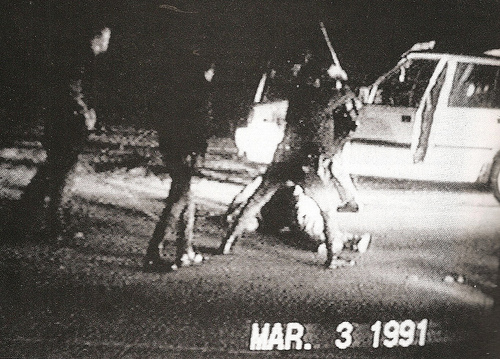
\includegraphics[width=0.4\textwidth]{figure/rodneyking.jpg}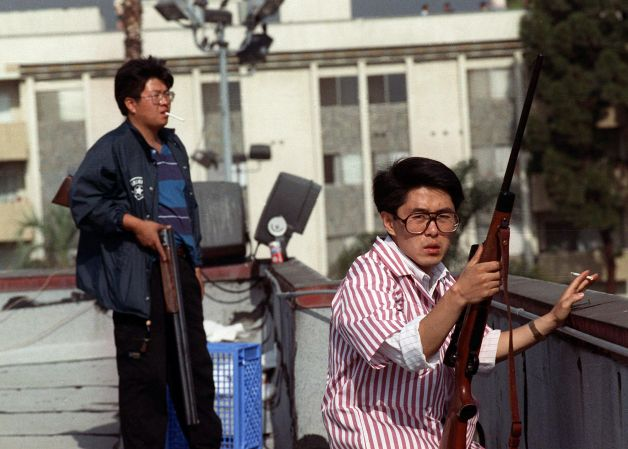
\includegraphics[width=0.4\textwidth]{figure/koreangrocer.jpg}\\
%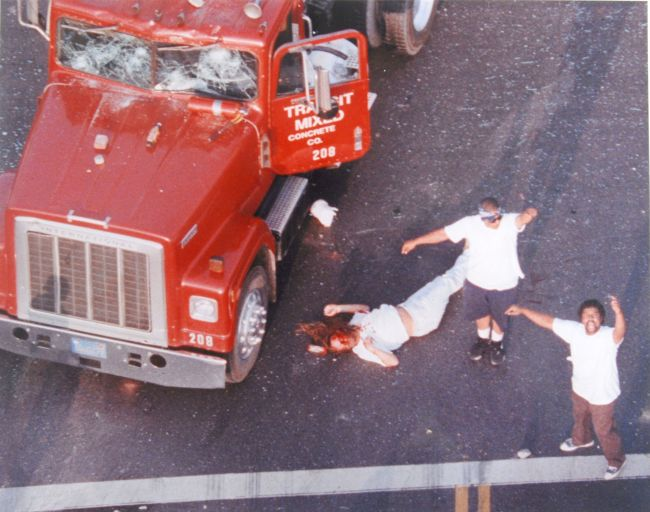
\includegraphics[width=0.4\textwidth]{figure/ReginaldDenny.jpg}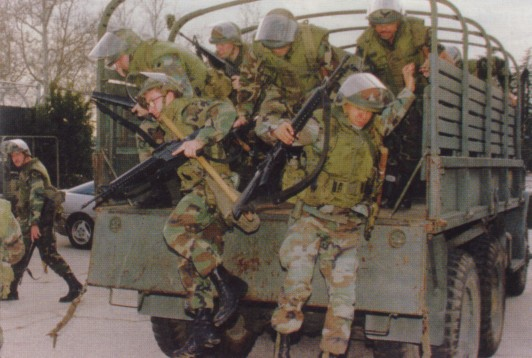
\includegraphics[width=0.4\textwidth]{figure/nationalguard.jpg}
%\end{center}
%
%\end{frame}
%%------------------------------------------------------------------------------
%
%
%%------------------------------------------------------------------------------
%\begin{frame}[fragile]
%\frametitle{Early 1990's Los Angeles}
%Then in 1994 there was a trial involving former NFL star O.J. Simpson.  He was accused of killing his ex-wife Nicole Brown Simpson and her friend Ron Goldman and later acquitted.  
%
%\begin{center}
%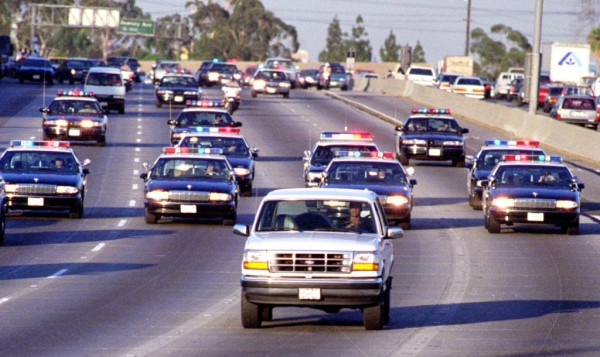
\includegraphics[width=0.6\textwidth]{figure/bronco.jpg}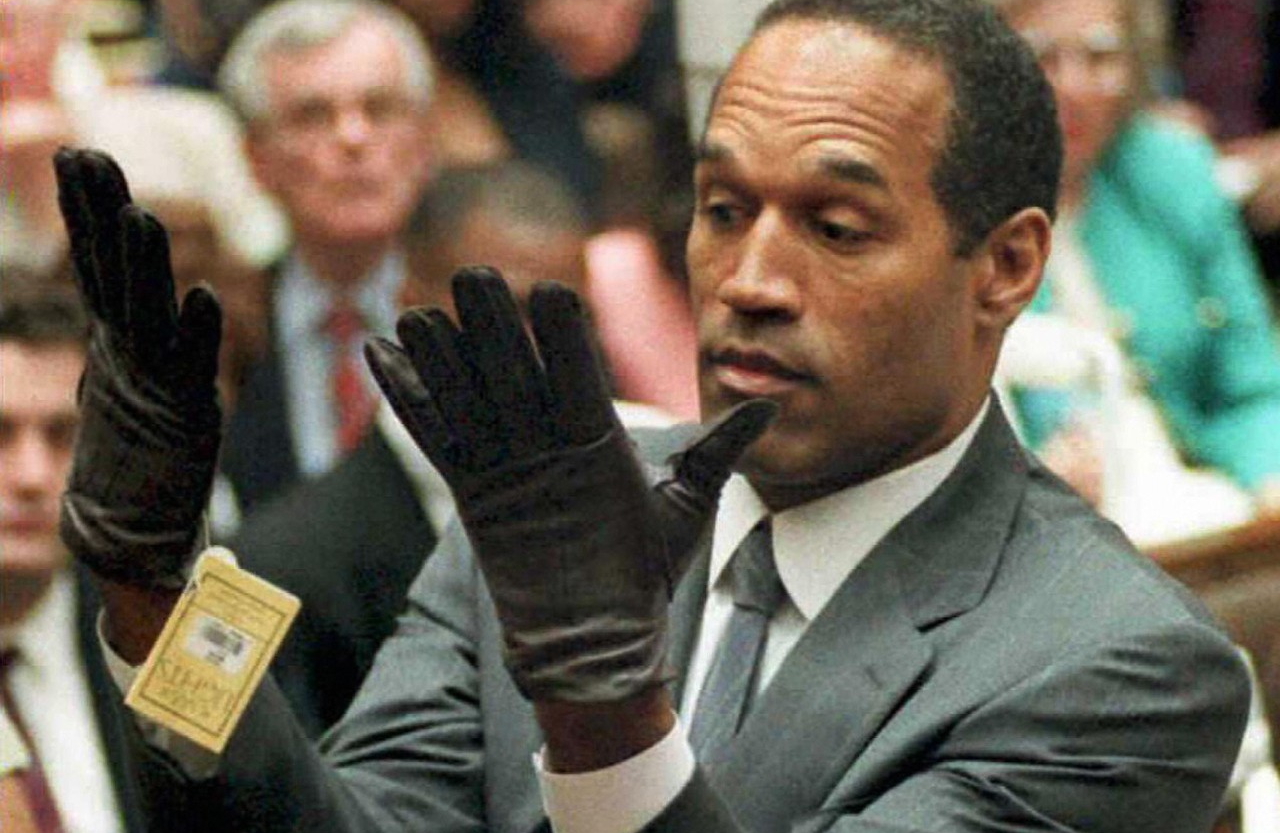
\includegraphics[width=0.4\textwidth]{figure/OJsimpson.png}
%\end{center}
%
%\end{frame}
%%------------------------------------------------------------------------------


%------------------------------------------------------------------------------
\begin{frame}[fragile]
\frametitle{Jury Selection}

Preview of next lecture:  In many trials a big issue is the \blue{racial makeup} of the jury.  

\vspace{0.25cm}

\pause Question: is there a way to figure out if there is a \blue{racial bias} in jury selection?  

\end{frame}
%------------------------------------------------------------------------------


%------------------------------------------------------------------------------
\begin{frame}[fragile]
\frametitle{Jury Selection}
Say we have a juror pool (registered voters) where the racial breakdown is:


\begin{center}
\begin{tabular}{l||cccc|c}
Race & White & Black & Hispanic & Other & Total \\ 
\hline
Registered Voters & 72\% & 7\% & 12\% & 9\% & 100\%\\ 
\textcolor{white}{Representation} & \textcolor{white}{0} & \textcolor{white}{0} & \textcolor{white}{0} & \textcolor{white}{100} & \textcolor{white}{$n=100$} \\ 
\end{tabular}
\end{center}

\white{blah blah}


\end{frame}
%------------------------------------------------------------------------------


%------------------------------------------------------------------------------
\begin{frame}[fragile]
\frametitle{Jury Selection}
If we pick $n=100$ jurors \blue{at random} (i.e. unbiasedly), we \blue{expect} the breakdown of counts to be:

\begin{center}
\begin{tabular}{l||cccc|c}
Race & White & Black & Hispanic & Other & Total \\ 
\hline
Registered Voters & 72\% & 7\% & 12\% & 9\% & 100\%\\ 
Representation & 72 & 7 & 12 & 9 & $n=100$ \\ 
\end{tabular}
\end{center}

\white{blah blah}

\end{frame}
%------------------------------------------------------------------------------


%------------------------------------------------------------------------------
\begin{frame}[fragile]
\frametitle{Jury Selection}
Say we \blue{observe} the following counts: \white{blah blah blah blah blah blah blah blah blah blah blah blah}

\begin{center}
\begin{tabular}{l||cccc|c}
Race & White & Black & Hispanic & Other & Total \\ 
\hline
Registered Voters & 72\% & 7\% & 12\% & 9\% & 100\%\\ 
Representation & 0 & 0 & 100 & 0 & $n=100$ \\ 
\end{tabular}
\end{center}

\pause Fairly obvious bias in juror selection!

\end{frame}
%------------------------------------------------------------------------------


%------------------------------------------------------------------------------
\begin{frame}[fragile]
\frametitle{Jury Selection}
But what about the following?  Is there a bias?  i.e. a non-random mechanism at play?

\begin{center}
\begin{tabular}{l||cccc|c}
Race & White & Black & Hispanic & Other & Total \\ 
\hline
Registered Voters & 72\% & 7\% & 12\% & 9\% & 100\%\\ 
Representation & 75 & 6 & 11 & 8 & $n=100$ \\ 
\end{tabular}
\end{center}

\white{blah blah}

\end{frame}
%------------------------------------------------------------------------------


%------------------------------------------------------------------------------
\begin{frame}[fragile]
\frametitle{Next Two Lectures}

Chi-square tests are used to compare \blue{expected} counts with \blue{observed} counts.

\vspace{0.25cm}

\pause Two tests we'll see:
\begin{itemize}
\item Goodness-of-fit tests:  for frequency tables
\item Tests for independence:  for contingency/two-way tables
\end{itemize}

\end{frame}
%------------------------------------------------------------------------------

\end{document}










